\begin{activity} \label{A:10.4.10} 
\ba
\item Evaluate the function and its partial derivatives at $(x_0,y_0)
  = (1,1)$;  that is, find $f(1,1)$, $f_x(1,1)$, and $f_y(1,1)$.

\item We know one point on the tangent plane;  namely, the tangent
  plane agrees with the graph of the function at the point $(x_0,
  y_0)$.  Use this observation to determine $z_0$ in the expression
  $z = z_0 + a(x-x_0) + b(y-y_0)$.

\item Sketch the traces of the function for $y=y_0=1$ and $x=x_0=1$
  below in Figure \ref{F:10.4.traces}.  

  \begin{figure}[ht]
    \begin{center}
      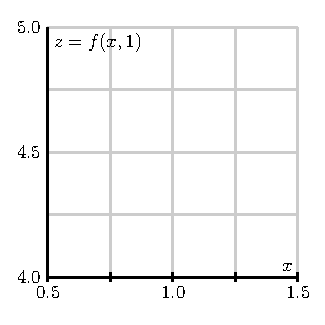
\includegraphics{figures/fig_10_4_tangent_trace_y.eps}
      \hspace*{20pt}
      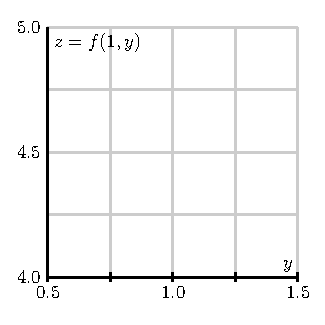
\includegraphics{figures/fig_10_4_tangent_trace_x.eps}
    \end{center}
    \caption{The traces of $f(x,y)$ with $y=y_0=1$ and $x=x_0=1$.}
    \label{F:10.4.traces}
  \end{figure}

\item Write the equation of the tangent line of the trace with $y=1$
  at the point $x_0=1$.  

\item Figure \ref{F:10.4.tangent.traces} shows the traces of the
  function and the traces of the tangent plane.  Explain how the
  tangent line of the trace of $f$, whose equation you found in the
  last part of this 
  activity, is related to the tangent plane.  How does this
  observation help you determine the constant $a$ in the expression
  for the tangent plane $z
  = z_0+a(x-x_0) + b(y-y_0)$?  

  \begin{figure}[ht]
    \begin{center}
      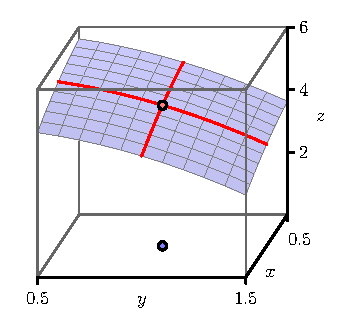
\includegraphics{figures/fig_10_4_tangent_5.eps}
      \hspace*{20pt}
      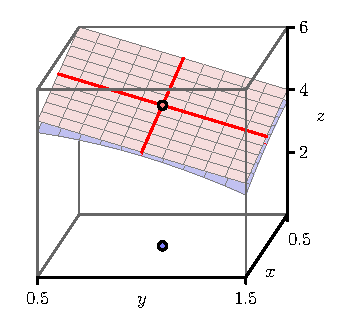
\includegraphics{figures/fig_10_4_tangent_6.eps}
    \end{center}
    \caption{The traces of $f(x,y)$ and the tangent plane.}
    \label{F:10.4.tangent.traces}
  \end{figure}

\item In the same way, write the equation of the tangent line of the
  trace with $x=1$ at the point $y_0=1$.  Explain how this tangent
  line is related to the tangent plane and use this observation to
  determine the constant $b$ in the expression for the tangent plane
  $z=z_0+a(x-x_0) + b(y-y_0)$.

\item Write the equation $z=z_0 + a(x-x_0) + b(y-y_0)$ of the tangent
  plane to the graph of $f(x,y)=6-x^2/2 - y^2$ at the point
  $(x_0,y_0)=(1,1)$. 

\ea

\end{activity}
\aftera
